\setlength{\columnsep}{3pt}
\begin{flushleft}

\bigskip

\paragraph{What are logs in Linux?}
\begin{itemize}
	\item Linux logs provide a timeline of some important events.
	\item Logs are used for troubleshooting issues \& problems. 
	\item Location of log files: \textbf{/var/log} directory. 
	\item There are Linux logs for: \textbf{system, kernel, package managers, boot processes, Xorg, Apache, MySQL}, etc
	\item Sample log entry from \textbf{/var/log/messages} file:
	
	\begin{figure}[h!]
		\centering
		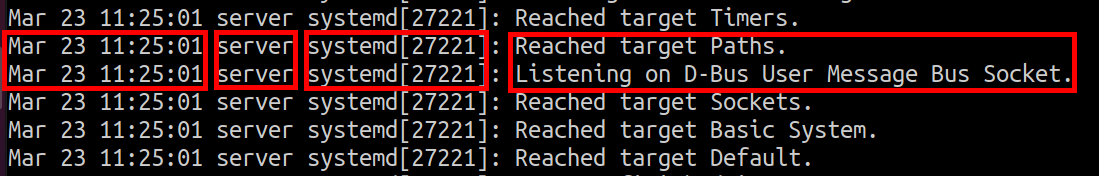
\includegraphics[scale=0.35]{content/chapter16/images/logs_entry.png}
		\caption{Sample log}
		\label{fig:log}
	\end{figure}
	Understanding log entry:
	\begin{itemize}
		\item Column 1: \textbf{Timestamp}
		\item Column 2: The \textbf{hostname of the server where the log is generated}
		\item Column 3: The \textbf{daemon generating the logs}
		\item Column 4: The \textbf{log message}
	\end{itemize}
	
\end{itemize}

\end{flushleft}
\newpage


